%%%%%%%%%%%%%%%%%%%%%%%%%%%%%%%%%%%%%%%%%%%%%%%%
% E.Pinault-Bigeard - e.pinault-bigeard@upsti.fr
% http://s2i.pinault-bigeard.com
% CC BY-NC-SA 2.0 FR - http://creativecommons.org/licenses/by-nc-sa/2.0/fr/
%%%%%%%%%%%%%%%%%%%%%%%%%%%%%%%%%%%%%%%%%%%%%%%%
\documentclass[11pt]{article}
%%%%%%%%%%%%%%%%%%%%%%%%%%%%%%%%%%%%%%%%%%%%%%%%
% Package UPSTI_Document
%%%%%%%%%%%%%%%%%%%%%%%%%%%%%%%%%%%%%%%%%%%%%%%%
%%%%%%%%%%%%%%%%%%%%%%%%%%%%%%%%%%%%%%%%%%%%%%%%
% Package UPSTI_Document
%%%%%%%%%%%%%%%%%%%%%%%%%%%%%%%%%%%%%%%%%%%%%%%%
\usepackage{subcaption}
\usepackage[usenames, svgnames, dvipsnames]{xcolor}
\usepackage{UPSTI_Document}
\usepackage{pgfplots}
\usepackage{import}
\definecolor{darkspringgreen}{rgb}{0.09, 0.45, 0.27}

\newcommandx*{\dessinRepereFigGeo}[5][1=\vx{},2=\vy{},3=\vz{},4=,5=0]
	{
		\draw [->,very thick] (0,0) -- (1,0) ;
		\draw [->,very thick] (0,0) -- (0,1) ;
    \fill[white] (0,0) circle (0.13);
    \draw [->,very thick] (0,0) circle (0.13);
    \ifnumequal{#5}{0} {% z vers nous
      \fill[black] (0,0) circle (0.03);
      \draw [->,thick] (0,0) circle (0.04);
    }{% z vers la feuille
  		\begin{scope} [rotate=45]
  			\draw [-,thick] (0,-0.12) -- (0,0.12) ;
  			\draw [-,thick] (-0.12,0) -- (0.12,0) ;
  		\end{scope}
    }
		\draw [anchor=north west] (1.1,0) node {${#1}$};
		\draw [anchor=south west] (0,1.1) node {${#2}$};
		\draw [anchor=north east] (-0.1,0) node {${#3}$};
		\draw [anchor=north west] (-0.1,-0.1) node {${#4}$};
	}

	\usepackage{array}
	\newcolumntype{L}[1]{>{\raggedright\let\newline\\\arraybackslash\hspace{0pt}}m{#1}}
	\newcolumntype{C}[1]{>{\centering\let\newline\\\arraybackslash\hspace{0pt}}m{#1}}
	\newcolumntype{R}[1]{>{\raggedleft\let\newline\\\arraybackslash\hspace{0pt}}m{#1}}

	\usepackage{pifont}% http://ctan.org/pkg/pifont
\newcommand{\cmark}{\color{green}\ding{51}}%
\newcommand{\xmark}{\color{red}\ding{55}}%
\newcommand{\fmark}{\ding{229}}%
\newcommand{\itemc}{\item[\cmark]}%
\newcommand{\itemx}{\item[\xmark]}%
\newcommand{\itemf}{\item[\fmark]}%

\usepackage{multirow}
\usepackage{placeins}

%---------------------------------%
% Paramètres du package
%---------------------------------%

% Version du document (pour la compilation)
% 1: Document prof
% 2: Document élève
% 3: Document à publier
\newcommand{\UPSTIidVersionDocument}{1}


% Classe
% 1: PTSI				6: PSI*			11: TSI2		16: Spé
% 2: PT	(par défaut)	7: MPSI			12: ATS
% 3: PT*				8: MP			13: PC
% 4: PCSI				9: MP*			14: PC*
% 5: PSI				10: TSI1		15: Sup
%\newcommand{\UPSTIidClasse}{2}



% Matière
% 1: S2I (par défaut)    2: IPT     3: TIPE
% 6: Vie au lycée
\newcommand{\UPSTIidMatiere}{0}
\newcommand{\UPSTIintituleMatiere}{Réseaux}
\newcommand{\UPSTIsigleMatiere}{Réseaux}
% Type de document
% 0: Custom*				7: Fiche Métho de			14: Document Réponses
% 1: Cours (par défaut)		8: Fiche Synthèse    		15: Programme de colle
% 2: TD     				9: Formulaire
% 3: TP						10: Memo
% 4: Colle					11: Dossier Technique
% 5: DS						12: Dossier Ressource
% 6: DM						13: Concours Blanc
% * Si on met la valeur 0, il faut décommenter la ligne suivante:
%\newcommand{\UPSTItypeDocument}{Custom}
\newcommand{\UPSTIidTypeDocument}{1}

% Titre dans l'en-tête

% Affichage personnalisé de la classe
\newcommand{\UPSTIclasse}{GEII}

% Variante utilisée
\newcommand{\UPSTIvariante}{5}

% Titre dans l'en-tête

\newcommand{\UPSTItitreEnTete}{Réseaux}
%\newcommand{\UPSTItitreEnTetePages}{}
\newcommand{\UPSTIsousTitreEnTete}{Introduction aux réseaux Ethernet}


% Titre
%\newcommand{\UPSTItitrePreambule}{Automatisme industriel}
%\newcommand{\UPSTItitre}{Introduction aux réseaux Ethernet}

% Durée de l'activité (pour DS, DM et TP)
%\newcommand{\UPSTIduree}{3h30}

% Note de bas de première page
%\newcommand{\UPSTInoteBasDePremierePage}{Geoffrey Vaquette}
% Numéro (ajoute " n°1" après DS ou DM)
%\newcommand{\UPSTInumero}{1}

% Numéro chapitre
%\newcommand{\UPSTInumeroChapitre}{1}

% En-tête customisé
%\newcommand{\UPSTIenTetePrincipalCustom}{UPSTIenTetePrincipalCustom}

% Message sous le titre
%\newcommand{\UPSTImessage}{Message sous le titre}


% Référence au programme
%\newcommand{\UPSTIprogramme}{\EPBComp \EPBCompP{B1-02}, \EPBCompP{B2-49}, \EPBCompS{B2-50}, \EPBCompS{B2-51}, \EPBCompP{C1-07}, \EPBCompP{C1-08}}

% Si l'auteur n'est pas l'auteur par défaut
%\renewcommand{\UPSTIauteur}{WWOOOOOOWW}

% Si le document est réalisé au nom de l'équipe
%\newcommand{\UPSTIdocumentCollegial}{1}

% Source
\newcommand{\UPSTIsource}{A. Juton, J. Maillefert, G. Vaquette}

% Version du document
\newcommand{\UPSTInumeroVersion}{0.1}

%-----------------------------------------------
\UPSTIcompileVars		% "Compile" les variables
%%%%%%%%%%%%%%%%%%%%%%%%%%%%%%%%%%%%%%%%%%%%%%%%


%%%%%%%%%%%%%%%%%%%%%%%%%%%%%%%%%%%%%%%%%%%%%%%%
% Début du document
%%%%%%%%%%%%%%%%%%%%%%%%%%%%%%%%%%%%%%%%%%%%%%%%
\begin{document}
\UPSTIbuildPage

\tableofcontents


\section{Qu'est-ce qu'un réseau ? Qu'est-ce qu'internet ?}
\subsection{Un réseau}

De tout temps, les humains ont ressenti et ressentent le besoin de communiquer.
Les méthodes dont nous nous servons pour partager idées et informations changent et évoluent sans cesse. Si le réseau humain se limitait autrefois à des conversations en face à face, aujourd'hui les découvertes en matière de supports étendent sans cesse la portée de nos communications. De la presse écrite à la télévision, chaque innovation a développé et amélioré nos moyens de communication.

Avant de commencer ce cours sur les réseaux informatiques, nous devons définir ce qu'est un réseau.
% A retenir
\UPSTIdefinition[Réseau]{\UPSTIlignesACompleter{ Un réseau désigne un ensemble de relations. Définir un réseau, c'est donc définir des \textbf{liens}. D'une façon plus concrète, on dira : \textbf{Un réseau est un groupe d'entités en communication}}}

Une \textit{entité} peut être de tout type. Dans le cas d'un réseau social, les entités sont les personnes appartenant à un groupe social. Dans le cas d'un réseau informatique, les entités sont les appareil informatiques connectés ensembles.

En résumé, parler de réseau c'est simplement parler d'entités qui communiquent. La problématique de ce cours pourrait donc s'écrire :

\textbf{Comment faire en sorte que différents composants informatiques s'échangent des informations ? }

\subsection{Internet}

Ethymologiquement, Internet vient de \textit{inter} (entre) et \textit{net} (réseau). Il s'agit donc d'une connexion de multiples réseaux entre eux.

\UPSTIdefinition[Internet]{
Internet est un ensemble de réseaux interconnectés à l'échelle internationale qui échangent des informations selon des normes communes en utilisant des câbles téléphoniques, des câbles à fibre optique, des transmissions sans fil et des liaisons par satellite.
}



\subsection{Les protocoles}
Pour pouvoir donner une information à quelqu'un, il faut être capable de le joindre mais également de parler la même langue que lui (ou en tout cas que les différents intermédiaires comprennent leurs langues respectives).

En informatique, on ne parle pas de langue mais de protocole. Les machines communiquent en respectant un même protocole.

\UPSTIaRetenir{Les protocoles de communication définissent les "rêgles" que doivent respecter les machines pour communiquer.}

\section{Le matériel}
\subsection{Les supports de communication}
Pour transférer une information, il faut un support. Dans le cas d'une communication entre humain, il s'agit de l'air : les vibrations sonores se déplacent dans l'air pour parvenir jusqu'à la destination.

Dans le cas des réseaux informatiques, il existe une multitude de supports. Nous verrons ici les principaux : ceux que nous rencontrerons le plus dans ce module et ceux que l'on rencontre le plus souvent autour de nous.

\subsubsection{Les supports filaires}

\paragraph{Les câbles Ethernet}
C'est le câble le plus répandu pour relier des machines sur des réseaux de moyenne ou petites tailles.

Un câble Ethernet est un ensemble de 4 paires torsadées (Figure~\ref{fig:cableEthernet}).

Dans la configuration la plus simple, les paires oranges et vertes sont utilisées pour la tranmission des données, les deux autres paires ne sont pas utilisées.

Concrètement, lorsque deux machines sont reliées par un câble Ethernet, l'une d'elle émet sur une paire torsadée et écoute sur l'autre ; la deuxième machine fait l'inverse. Le signal Tx est utilisé pour \textbf{T}ransmettre et le signal Rx est utilisé pour \textbf{R}ecevoir. C'est pourquoi on utilise des câbles dits \textit{croisés} pour relier deux ordinateurs ensembles : Les broches Tx d'un élément sont reliées aux Rx du deuxième et inversement.

Les câbles droits sont utilisés pour relier les ordinateurs à des organes propres au réseau comme un concentrateur dont les broches Tx et Rx sont inversées.

\begin{figure}
\centering
  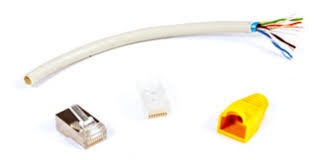
\includegraphics[width=.3\textwidth]{images/materiel/cableEthernet}
  \caption{Câble Ethernet et son interface RJ45}
  \label{fig:cableEthernet}
\end{figure}

\UPSTIremarque{On dit parfois \textit{câble RJ45}. Il s'agit d'un abus de langage car \textbf{RJ45} désigne l'interface (embout) du câble.}

\paragraph{La fibre optique}
Pour relier des réseau entre eux, on utilise de plus en plus la fibre optique. Un tel câble utilise la lumière comme moyen de propagation de l'information. Vous verrez son principe de fonctionnement plus en détail en cours de physique S3.

La fibre optique permet de bien plus forts débits qu'un cable Ethernet en cuivre (plusieurs Terabit par seconde contre plusieurs Gb/s pour un cable Ethernet). Les connexions intercontinentales sont notamment réalisé avec une fibre optique.

Comme pour un support en cuivre, la fibre optique subit une atténuation avec la distance. Afin de permettre au signal de traverser de très longues distances (l'atlantique par exemple), on pose régulièrement des répéteur qui reçoivent le signal, l'amplifient, puis le répète.

La Figure~\ref{fig:poseFibre} illustre la pose d'un câble de fibre optique sous-marin.

\begin{figure}[h]
\centering
  \definecolor{Gray}{gray}{0.9}
\definecolor{Gray2}{gray}{0.7}
\newcolumntype{a}{>{\columncolor{Gray}}c}
\newcolumntype{b}{>{\columncolor{Gray2}}c}

\begin{tabular}{|a|a|a|a|a|a|a|a|c|c|c|c|c|c|c|c|c|c|c|c|c|c|b|b|b|b|b|b|b|b|b|b|b|a|a|a|a|}
\hline
  &&&&&&&&&&&&&&&&&&&&&&&&&&\multicolumn{3}{|b|}{\dots}&&&&&&&& \\\hline
  \multicolumn{7}{|a|}{}          & S &\multicolumn{6}{c|}{Adresse}               &\multicolumn{6}{c|}{Adresse}             & \multicolumn{2}{c|}{L}  &\multicolumn{11}{b|}{}     &\multicolumn{4}{a|}{C}  \\
  \multicolumn{7}{|a|}{Préambule} & F &\multicolumn{6}{c|}{MAC}                   &\multicolumn{6}{c|}{MAC}                 & \multicolumn{2}{c|}{/}  &\multicolumn{11}{b|}{Data}  &\multicolumn{4}{a|}{R}  \\
  \multicolumn{7}{|a|}{}          & D &\multicolumn{6}{c|}{\textbf{destinataire}} &\multicolumn{6}{c|}{\textbf{expediteur}} & \multicolumn{2}{c|}{T}  &\multicolumn{11}{b|}{}      & \multicolumn{4}{a|}{C}  \\\hline
  \multicolumn{7}{|a|}{7 octets}  & 1o &\multicolumn{6}{c|}{6 octets}             &\multicolumn{6}{c|}{6 octets}            & \multicolumn{2}{c|}{2o}  &\multicolumn{11}{b|}{De 46 à 1500 octets}      &\multicolumn{4}{a|}{4o}  \\\hline

\end{tabular}

  \caption{Pose d'un câble de fibre optique sous-marin (Source : Le Monde)}
  \label{fig:poseFibre}
\end{figure}

\subsubsection{Supports sans fil}
\paragraph{Wi-Fi}
A l'échelle locale, le support sans-fil le plus utilisé est sans doute la connexion Wi-Fi. Il s'agit d'une transmission par ondes électromagnétiques à des fréquences entre \SI{2.4}{GHz} et \SI{2.4935}{GHz}.

La connexion Wi-Fi a un débit théorique inférieur à une connexion Ethernet mais permet la mobilité des organes connectés.

\subsection{Les organes}
\label{sec:organes}
\subsubsection{La carte réseau}
\label{sec:CarteReseau}
Un ordinateur (ou n'importe quel appareil informatique) communique via sa carte réseau. C'est elle qui fait l'interface entre l'ordinateur et le réseau en lui-même.

Lorsque votre ordinateur communique sur le réseau, c'est en réalité sa carte réseau qui le fait. De même, les paquets (messages) sont adressés à cette carte réseau.

Chaque carte réseau possède un identifiant \textbf{unique} appelé \textbf{adresse MAC}. C'est sa carte d'identité, ce qui l'identifie au sein d'un réseau. Nous en reparlerons quand nous parlerons du protocole de communication Ethernet.

\begin{figure}[h]
\centering
  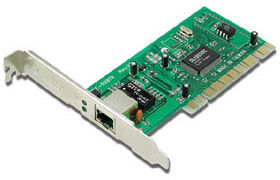
\includegraphics[width=.4\textwidth]{images/materiel/carteReseau}
  \caption{Carte réseau}
  \label{fig:carteReseau}
\end{figure}

\subsubsection{Concentrateur (hub)}
\label{sec:concentrateur}
Un concentrateur est un dispositif qui permet de relier différents organes (ordinateurs) entre-eux. Chaque organe est relié sur un port (prise RJ45) différent. On peut le voir comme une simple "multi-prise" qui se contente d'envoyer tout ce qu'elle reçoit sur un port sur les autres ports.

Par exemple, si quatre ordinateurs sont connectés sur les ports 1, 2, 3 et 4 et que l'ordinateur branché sur le port 4 envoie un paquet à celui connecté sur le port 2, le hub le transmettra sur les ports 1, 2 et 3 sans se soucier du destinataire du message.

\subsubsection{Commutateur (switch)}
\label{sec:commutateur}
Un commutateur sert également à relier différents organes entre-eux au sein d'un réseau. Cependant, contrairement au concentrateur, le commutateur ne recopie pas tous les messages qu'il reçoit sur tous les ports. En effet, il n'enverra le paquet uniquement au port sur lequel est connecté son destinataire.

En reprenant l'exemple précédent, lorsque l'ordinateur connecté au port 4 désire envoyer un paquet à celui connecté au port 2, le commutateur transmettra ce message sur le port 2 et non sur les autres ports.

Pour identifier les éléments connectés sur ses ports, le commutateur utilise l'adresse MAC (l'identifiant unique attribué aux cartes réseaux).

\subsubsection{Routeur}
\label{sec:routeur}
Un routeur, quant à lui, permet non seulement de connecter des organes entre-eux, mais il fait également le lien entre deux réseaux différents. L'exemple le plus parlant est sûrement la box internet que chacun à chez soi. Elle permet de relier les différents ordinateur du domicile entre-eux et permet également à ces ordinateur d'accéder à un réseau bien plus étendu : internet.


\subsection{On récapitule}

Le tableau~\ref{tab:materiel} (issu du site OpenClassRooms) regroupe les différents materiels abordés et leur fonctions principales.

\begin{table}[h!t]
\centering
  \begin{tabular}{l|p{.6\textwidth}}
  \textbf{Matériel} & \textbf{Fontion} \\\hline
  Carte réseau & La carte réseau est le matériel de base indispensable, qui traite tout au sujet de la communication dans le monde du réseau.\\\hline

Concentrateur (hub) & Le concentrateur permet de relier plusieurs ordinateurs entre eux, mais on lui reproche le manque de confidentialité. On peut le voir comme une simple «multi-prise» Ethernet. \\\hline

Commutateur (switch) & Le commutateur fonctionne comme le concentrateur, sauf qu'il transmet des données aux destinataires en se basant sur leurs adresses MAC (adresses physiques). Chaque machine reçoit seulement ce qui lui est adressé.\\\hline

Routeur & Le routeur permet d'assurer la communication entre différents réseaux pouvant être fondamentalement différents (réseau local et Internet).\\\hline

Répéteur& Le répéteur reçoit des données par une interface de réception et les renvoie plus fort par l'interface d'émission. On parle aussi de relais en téléphonie et radiophonie.\\
\end{tabular}

  \caption{Récapitulatif des matériels abordés}
  \label{tab:materiel}
\end{table}


\section{Topologies des réseaux}
Maintenant que nous connaissons le matériel nécessaire pour établir une connexion, nous pouvons voir les différentes manières possible de les connecter entre-eux. La façon dont les appareils sont connectés entre-eux est appelée \textbf{topologie}. On peut différencier deux types de topologies.

\UPSTIdefinition{
  La \textbf{topologie physique} désigne la configuration spatiale du réseau. C'est la façon dont les organes sont connectés \textbf{physiquement}.
}
\UPSTIdefinition{
  La \textbf{topologie logique} désigne quant à elle la manière dont les données transitent dans les câbles.
}

\subsection{Quelques topologies physiques classiques}
\begin{figure}[h!t]
  \centering
  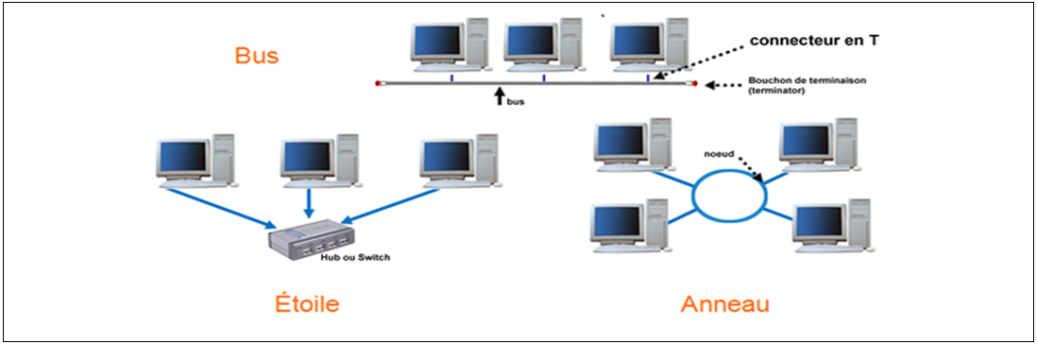
\includegraphics[width=.7\textwidth]{images/topologies/reseau_topologies}
  \caption{Trois exemples de topologies de réseau.}
  \label{fig:res_topo}
\end{figure}
\subsubsection{Topologie en bus}
\begin{figure}[h!]
  \centering
  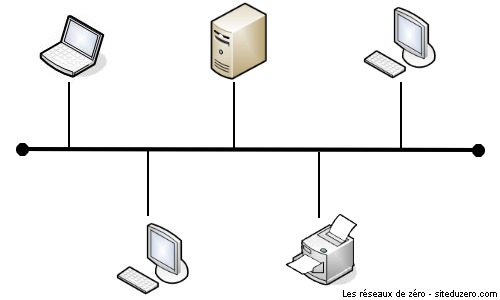
\includegraphics[width=.4\textwidth]{images/topologies/topologieBus}
  \caption{Topologie en BUS}
  \label{fig:topoBus}
\end{figure}
Une topologie en bus (Figure~\ref{fig:topoBus}) est l'organisation la plus simple d'un réseau. Dans une topologie en bus tous les ordinateurs sont reliés à une même ligne de transmission par l'intermédiaire d'un seul câble. Le mot "bus" désigne la ligne physique qui relie les machines du réseau.

Cette topologie a pour avantages d'être {facile à mettre en oeuvre} et de fonctionner facilement, par contre elle est extrêmement {vulnérable} étant donné que si l'une des connexions est défectueuse, c'est l'ensemble du réseau qui est affecté.

Cette topologie est obsolète dans les réseaux de données mais couramment utilisé dans les réseaux de terrain (automates industriels ou voitures par exemple).

\subsubsection{Topologie en anneau}

Dans un réseau en topologie en anneau, les ordinateurs sont reliés sur une bouble. On peut le voir comme un réseau en bus dont on a relié les extrémités. Comme pour le réseau en BUS, les composants ne peuvent pas communiquer en même temps car cela créerait une collision de données. Dans une topologie en anneau, les appareils communiquent chacun leur tour en échangeant un jeton (\textit{token})

En réalité les ordinateurs d'un réseau en topologie anneau ne sont pas reliés en boucle, mais sont reliés à un répartiteur (appelé MAU, Multistation Access Unit) qui gère la communication entre les différents composants.

\subsubsection{Topologie en étoile}
\begin{figure}[h!]
  \centering
  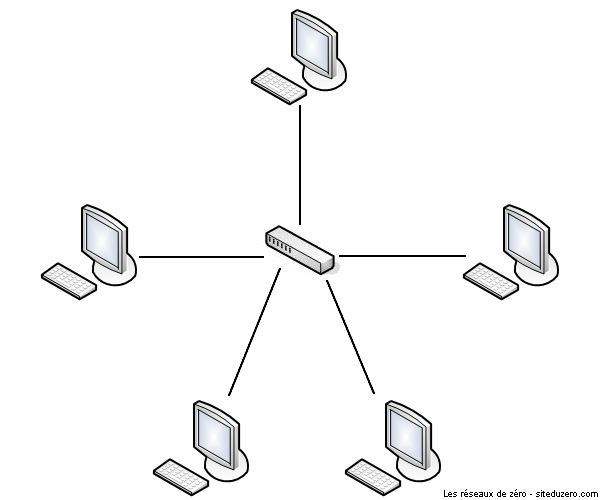
\includegraphics[width=.4\textwidth]{images/topologies/topologieEtoile}
  \caption{Topologie en étoile}
  \label{fig:topoEtoile}
\end{figure}
Dans une topologie en étoile (Figure~\ref{fig:topoEtoile}), les ordinateurs du réseau sont reliés à un noeud central. Chaque membre du réseau communique avec le noeud central au travers de sa propre connexion. Le noeud central fait le lien

Contrairement aux réseaux construits sur une topologie en bus, les réseaux suivant une topologie en étoile sont beaucoup moins vulnérables car on peut aisément retirer une des connexions en la débranchant du commutateur sans pour autant paralyser le reste du réseau.

\subsubsection{Topologie maillée}
\begin{figure}[h!]
  \centering
  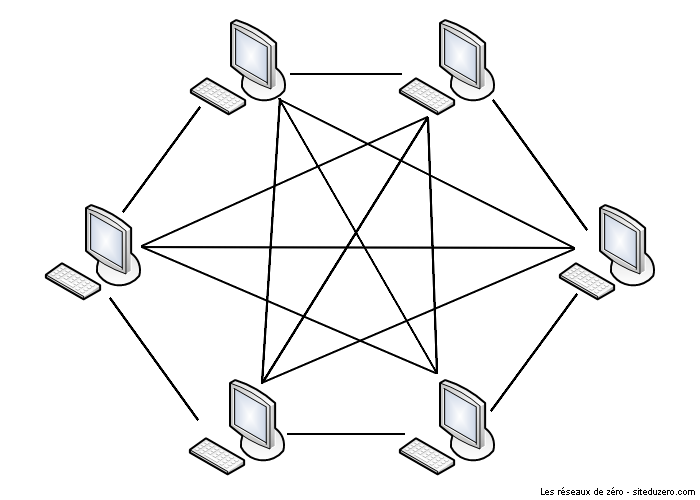
\includegraphics[width=.4\textwidth]{images/topologies/topologieMaillee}
  \caption{Topologie maillée}
  \label{fig:topoMaillee}
\end{figure}

Il s'agit de la topologie la plus robuste car tous les éléments sont connectés à tous les autres (Figure~\ref{fig:topoMaillee}). Chaque élément peut donc communiquer avec n'importe quel autre élément en utilisant la connexion propre. L'avantage d'une topologie maillée est sa robustesse aux pannes de raccordement. En effet, si le lien entre deux éléments est défectueux, cela n'aura une influence que sur la communication entre deux éléments. Les autres connexions sont toujours possibles. En passant par un intermédiaire, les deux éléments concernés peuvent d'ailleurs toujours communiquer.

En revanche, ce type de réseau impose un nombre de connexion considérable. Ce nombre est de $\frac{n(n-1)}{2}$ connexions, avec $n$ le nombre d'éléments connectés. Sur la Figure~\ref{fig:topoMaillee}, 6 éléments sont connectés, nécessitant $\frac{6 \times 5}{2} = 15$ câbles. Le calcul pour une institution ayant 500 machines donne alors un nombre de connexion de \num{124700}... C'est une architecture réseau qui convient donc dans des cas précis où la robustesse est primordiale et où la taille du réseau est suffisamment petite.

\subsubsection{Internet}

Internet est un ensemble de réseaux interconnecté. Il est chacun de ces réseaux a sa propre topologie (le plus souvent une topologie en étoile). Cette diversité de topologies et le fait que plusieurs chemins soient possibles font qu'internet a une topologie hybride.

\section{Le modèle OSI}
Au début des années 70, chaque constructeur a développé sa propre solution réseau autour d'architecture et de protocoles privés (SNA d'IBM, DECnet de DEC, DSA de Bull, TCP/IP du DoD,...) et il s'est vite avéré qu'il serait impossible d'interconnecter ces différents réseaux «propriétaires» si une norme internationale n'était pas établie. Cette norme établie par l'International Standard Organization (ISO) est la norme Open System Interconnection (OSI, interconnexion de systèmes ouverts).

Un système ouvert est un ordinateur, un terminal, un réseau, n'importe quel équipement respectant cette norme et donc apte à échanger des informations avec d'autres équipements hétérogènes et issus de constructeurs différents.

Le modèle de référence OSI est une représentation abstraite en couches servant de guide à la conception des protocoles réseau. Il divise le processus de réseau en sept couches logiques, chacune comportant des fonctionnalités uniques et se voyant attribuer des services et des protocoles spécifiques.

\begin{figure}[h!t]
  \centering
  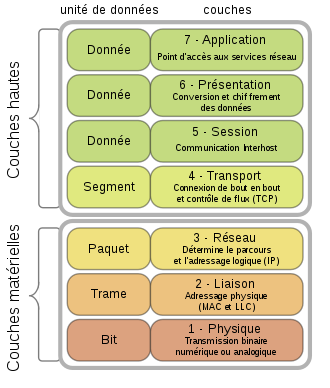
\includegraphics[height=.3\textheight]{images/osi/reseau_OSI}
  \caption{Les couches du modèle OSI}
  \label{fig:res_osi}
\end{figure}

\subsection{Les couches matérielles}
\label{sec:couches}
Ce sont celles qui assurent la liaison matérielle entre les organes. C'est cette couche qui s'assure qu'un paquet envoyé par un expéditeur $E$ arrive bien jusqu'au destinataire $D$.
\paragraph{Couche 1 : Couche physique}
\begin{description}
  \item [Nom : ] Couche Physique
  \item [Rôle : ] Offrir un support de transmission pour la communication
  \item [Rôle secondaire : ] Néant
  \item [Exemple de matériel associé : ] Concentrateur (cf \ref{sec:concentrateur})
\end{description}

\paragraph{Couche 2 : Couche liaison}
\begin{description}
  \item [Nom : ] Liaison de donnée
  \item [Rôle : ] Connecter les machines entre elles sur un réseau local.
  \item [Rôle secondaire : ] Détecter les erreurs de transmission.
  \item [Exemple de matériel associé : ] Commutateur (cf \ref{sec:commutateur})
\end{description}


\paragraph{Couche 3 : Couche réseau}
\begin{description}
  \item [Nom : ] Réseau
  \item [Rôle : ] Interconnecter les réseaux entre eux.
  \item [Rôle secondaire : ] Fragmenter les paquets.
  \item [Exemple de matériel associé : ] Routeur (cf \ref{sec:routeur})
\end{description}

\subsection{Les couches hautes}
Les couches hautes sont la plupart du temps logicielles. Elle permettent de faire le lien entre le paquet et l'utilisation que l'on fait de ce paquet. Dans les cours de ce module, nous nous intéresserons principalement aux couches matérielles ainsi qu'aux couches 4 et 7 et laisserons de côté les couches 5 et 6.

\paragraph{Couche 4 : Couche transport}
\begin{description}
  \item [Nom : ] Couche Transport
  \item [Rôle : ] gérer les connexions applicatives.
  \item [Rôle secondaire : ] garantir la connexion.
\end{description}


\paragraph{Couche 7 : Couche Application}
\begin{description}
  \item [Nom : ] Application
  \item [Rôle : ] ?
  \item [Rôle secondaire : ] ?
\end{description}
Cette couche représente l'application utilisant les paquets qui transitent sur le réseau. Elle n'a donc pas de rôle précis associé puisque cela dépendra de l'application.

\subsection{Le modèle OSI : une norme}
Le modèle OSI est une  norme, cela signifie qu'il définit des règles que les concepteurs de réseaux doivent suivre. Si chaque intervenant respecte la norme, alors le modèle OSI garantit le bon fonctionnement du réseau. Les matériels sont donc fabriqués selon cette norme afin d'assurer la compatibilité entre ces composants.

Ainsi, chaque couche doit remplir son rôle et uniquement son rôle. Deux règles générales entre les couches s'ajoutent :
\begin{itemize}
  \item Chaque couche est indépendante
  \begin{itemize}
    \item Les informations utilisées par une couche ne pourront pas être utilisées par une autre couche.
Par exemple, pour ceux qui connaissent déjà un peu le réseau, l'adresse IP qui est une adresse de couche 3 ne pourra pas être utilisée par une autre couche, sous peine de ne pas respecter le modèle OSI.
  \item Cela permet notamment de garantir l'évolution des communications dans le temps.
  \end{itemize}
  \item Chaque couche ne peut communiquer qu'avec une couche adjacente
  \begin{itemize}
    \item Pour envoyer une information, une appliction (couche 7) transmettra son paquet à la couche 6 qui le traitera et le passera à la couche 5 et ainsi de suite jusqu'à la couche 1.
    \item A la réception, le paquet remonte les couches jusqu'à la couche 7 de la l'application destinaire.
  \end{itemize}
\end{itemize}


\FloatBarrier
\section{Liaison Ethernet : les couches 1 et 2}
\subsection{Couche 0 : Transmission de données}
Pour la couche 0, la norme Ethernet définit les supports physiques possibles. En fonction de la norme suivie, différents débits
\begin{description}
  \item [10 BaseT : ] Paire torsadée \SI{100}{Mbit/s}
  \item [100 BaseT : ] Paire torsadée \SI{100}{Mbit/s}
  \item [1000 BaseT : ] Paire torsadée \SI{1}{Gbit/s}
  \item [1000 BaseX : ] Paire torsadée \SI{1}{Gbit/s}
  \item [Wifi] Liaison hertzienne \SI{54}{Mbit/s} à \SI{433}{Mbit/s}
\end{description}

Le format de la norme est également défini par la norme Ethernet. Par exemple, la norme 10 Bast-TX utilise le codage Manchester pour transmettre les données ainsi que l'horloge sur une seule paire de câble. La détection d'un 1 ou d'un 0 se fait alors en fonction du sens du front (montant ou descandante) et non du niveau sur un front d'horloge (voir Figure~\ref{fig:manchesterCode}).

\begin{figure}[h]
  \centering
  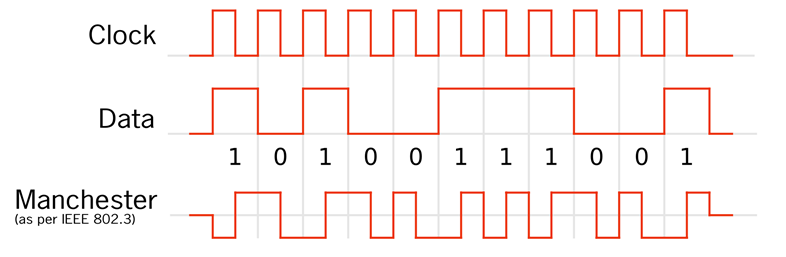
\includegraphics[width=.7\textwidth]{../../images/materiel/manchesterCode}
  \caption{Codage Manchester : L'horloge et les données sont envoyées sur le même signal}
  \label{fig:manchesterCode}
\end{figure}

\subsection{Couche 1 : Trame Ethernet}
\subsubsection{L'adresse MAC}
Comme discuté en section \ref{sec:CarteReseau}, chaque organe connecté au réseau possède une adresse MAC \textbf{unique} dans le monde. Chaque constructeur de carte réseau a un préfixe qui lui est attribué, puis il attribue à chaque matériel qu'il produit un code unique. Ainsi, théoriquement, tous les appareils connectés au réseaux possèdent une adresse MAC différente. On représente généralement une adresse MAC sous la forme hexadécimale pour des raisons évidentes de lisibilités. Par exemple, l'adresse MAC 00:1B:44:11:3A:B7 est décomposée dans le Tableau~\ref{tab:macExample}. Il est possible de retrouver le fabriquant d'une carte réseau via de nombreux site comme \url{https://macvendors.com/}.

\begin{table}[h!t]
\centering
  \begin{tabular}{ccc|ccc}
    octet 1 & octet 2 & octet 3 & octet 4 & octet 5 & octet 6\\
    \hline
    00      & 1B    &     44    & 11      &3A       &B7\\\hline
    \multicolumn{3}{c|}{Constructeur : }&\multicolumn{3}{c}{identifiant unique}\\
    \multicolumn{3}{c|}{SanDisk Corporation}&\multicolumn{3}{c}{}

  \end{tabular}
  \caption{Décomposition d'une adresse MAC : 00:1B:44:11:3A:B7}
  \label{tab:macExample}
\end{table}

\UPSTIaRetenir{L'adresse MAC est l'identifiant utilisé par le protocole Ethernet pour connaître le destinataire d'un message au sein d'un réseau.}
On peut faire une analogie entre l'adresse MAC et le nom que l'on écrirait sur une enveloppe pour la transmettre à une personne.

\begin{UPSTIactivite}
  Retrouver le constructeur de votre carte réseau à partir de son adresse MAC.
\end{UPSTIactivite}

\subsubsection{Décomposition d'une trame}

Lors de l'envoi d'une trame sur le réseau Ethernet, le premier niveau d'encapsulation correspond au protocole Ethernet. Dans un réseau local, c'est le protocole Ethernet qui définit le destinataire de la trame ainsi que son expéditeur. Tous deux sont identifiés par leur adresse MAC (adresse physique).
\begin{itemize}
  \item
\end{itemize}

\begin{description}
  \item [Préambule : ] Utilisation d’un modèle défini d’alternance de bits 1 et 0 pour synchroniser les appareils.
  \item [SFD : ]Délimitateur de début de Trame
  \item [MAC destination : ] Adresse de l'appareil destinataire
  \item [MAC expediteur : ] Adresse de l'appareil expediteur
  \item [Longueur/Type : ] Définit le type (ou parfois la longueur) de la trame.
  \begin{itemize}
    \item Dans le cas d'un envoi de trame TCP/IP, le type vaudra toujours \num{0x0800}
  \end{itemize}
  \item [Donnée encapuslées : ]Données à envoyer
  \item [CRC : ] La séquence de contrôle de trame contient une valeur de 4 octets créée par le périphérique qui envoie les données et recalculée par le périphérique de destination pour vérifier si les trames sont endommagées.
\end{description}

\UPSTIremarque{La taille d'une trame Ethernet doit être comprise entre 64 octets et 1564 octets. C'est pourquoi les données encapsulées ont une longueur allant de 46 à 1500 octets. Si on souhaite envoyer une trame plus courte, on ajoutera alors des données de bourrage (bits inutiles) pour atteindre la taille minimale.}

\begin{figure}
\centering
    \definecolor{Gray}{gray}{0.9}
\definecolor{Gray2}{gray}{0.7}
\newcolumntype{a}{>{\columncolor{Gray}}c}
\newcolumntype{b}{>{\columncolor{Gray2}}c}

\begin{tabular}{|a|a|a|a|a|a|a|a|c|c|c|c|c|c|c|c|c|c|c|c|c|c|b|b|b|b|b|b|b|b|b|b|b|a|a|a|a|}
\hline
  &&&&&&&&&&&&&&&&&&&&&&&&&&\multicolumn{3}{|b|}{\dots}&&&&&&&& \\\hline
  \multicolumn{7}{|a|}{}          & S &\multicolumn{6}{c|}{Adresse}               &\multicolumn{6}{c|}{Adresse}             & \multicolumn{2}{c|}{L}  &\multicolumn{11}{b|}{}     &\multicolumn{4}{a|}{C}  \\
  \multicolumn{7}{|a|}{Préambule} & F &\multicolumn{6}{c|}{MAC}                   &\multicolumn{6}{c|}{MAC}                 & \multicolumn{2}{c|}{/}  &\multicolumn{11}{b|}{Data}  &\multicolumn{4}{a|}{R}  \\
  \multicolumn{7}{|a|}{}          & D &\multicolumn{6}{c|}{\textbf{destinataire}} &\multicolumn{6}{c|}{\textbf{expediteur}} & \multicolumn{2}{c|}{T}  &\multicolumn{11}{b|}{}      & \multicolumn{4}{a|}{C}  \\\hline
  \multicolumn{7}{|a|}{7 octets}  & 1o &\multicolumn{6}{c|}{6 octets}             &\multicolumn{6}{c|}{6 octets}            & \multicolumn{2}{c|}{2o}  &\multicolumn{11}{b|}{De 46 à 1500 octets}      &\multicolumn{4}{a|}{4o}  \\\hline

\end{tabular}

  \caption{Décomposition d'une trame Ethernet}
\end{figure}

\subsubsection{Exemple d'envoi de trame : Concentrateur vs Commutateur}
\paragraph{Concentrateur}
Un concentrateur (souvent appelé hub) est un appareil appartenant à la couche 1 (physique, cf \ref{sec:couches}). Cela signifie que cet appareil n'a pas accès aux contenus des couches supérieures. Il est donc incapable d'identifier le destinataire d'un message.

Ainsi, lorsque l'on relie des appareil à l'aide d'un concentrateur (hub), les données envoyées sont transmises à tous les appareils connectés. Il appartiendra alors aux appareil de décider d'ouvrir ou non le message selon s'il leur est destiné ou non. La Figure~\ref{fig:trameConcentrateur} illustre l'envoi d'une trame par l'hôte H1 à l'hôte H6. Tous les appareils reçoivent la trame mais seul H6 l'ouvre car l'adresse MAC du message lui correspond. Cette animation est disponible à la section \href{https://static-course-assets.s3.amazonaws.com/NetEss/fr/index.html#3.4.1.3}{3.4.1.3} du cours netacad.

\UPSTIremarque{Puisque tous les appareils reçoivent la trame, l'utilisation d'un concentrateur peut être vue comme peu sécurisée. En effet, même s'il ne sont pas sensé l'ouvrir, n'importe quelle hôte pourrait avoir accès au message envoyé de H1 à H6.}



\paragraph{Commutateur}
Un commutateur (souvent appelé switch) est un appareil appartenant à la couche 2 (liaison, cf \ref{sec:couches}). Il a donc accès aux adresses MAC de la trame et est donc capable d'identifier le destinataire d'un message.

Ainsi, lorsque l'on relie des appareil à l'aide d'un commutateur (switch), ce dernier redirige le message uniquement vers son destinataire. La Figure~\ref{fig:trameCommutateur} illustre l'envoi d'une trame par l'hôte H1 à l'hôte H6. Puisqu'il connaît l'identité (adresse MAC) des hôtes connecté, le commutateur ne transmet le message que sur le câble connecté à H6. Cette animation est disponible à la section \href{https://static-course-assets.s3.amazonaws.com/NetEss/fr/index.html#3.4.2.1}{3.4.2.1} du cours netacad.

\UPSTIremarque{L'utilisation d'un switch (commutateur) présente deux avantages majeurs : \begin{itemize}
  \item Le réseau est moins encombré puisque les messages ne transitent pas inutilement vers des hôtes auxquels ils ne sont pas destinés.
  \item Il est \textit{a-priori} impossible pour les autres hôtes de lire le message puisque celui-ci n'arrive pas jusqu'à eux.
\end{itemize}}

\UPSTIremarque{L'étude de la table MAC d'un commutateur fait l'objet d'un exercice de TD.}

\begin{figure}[p]
\centering
\begin{subfigure}{\textwidth}
\centering
  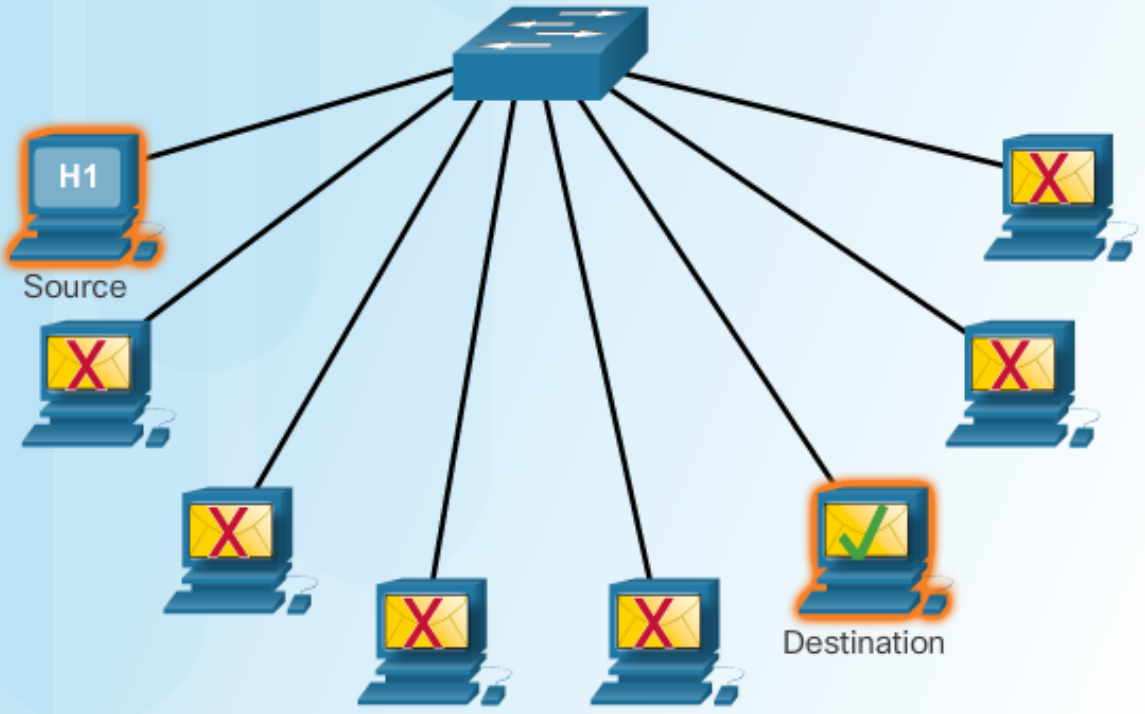
\includegraphics[width=.7\linewidth]{images/ethernet/concentrateurCroped}
  \caption{Envoi d'une trame par un concentrateur. Le message est transmis à tous les appreils connectés.}
  \label{fig:trameConcentrateur}
\end{subfigure}

\vspace{1cm}

  \begin{subfigure}{\textwidth}
  \centering
  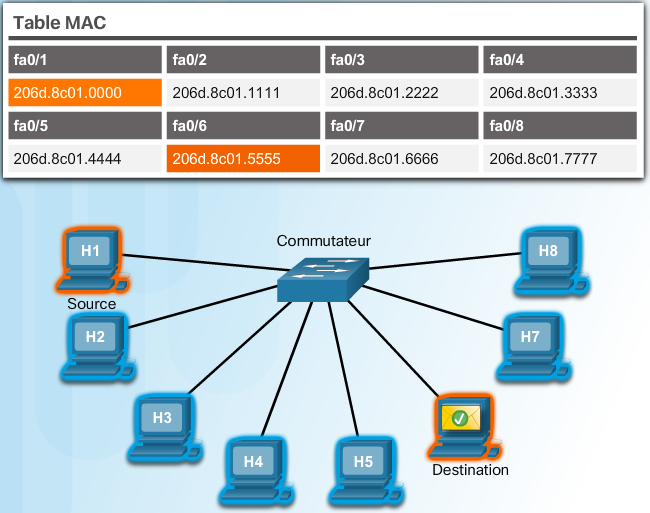
\includegraphics[width=.7\linewidth]{images/ethernet/communtateur}
  \caption{Envoi d'une trame par un commutateur. Le message est transmis uniquement à son destinataire.}
  \label{fig:trameCommutateur}
  \end{subfigure}
  \caption{Concentrateur vs Commutateur}
\end{figure}


%\UPSTIobjectif{Durant cette activité, nous allons analyser une trame pour l'envoi d'informations sur une étiquette.}



\end{document}
